164. \begin{figure}[ht!]
\center{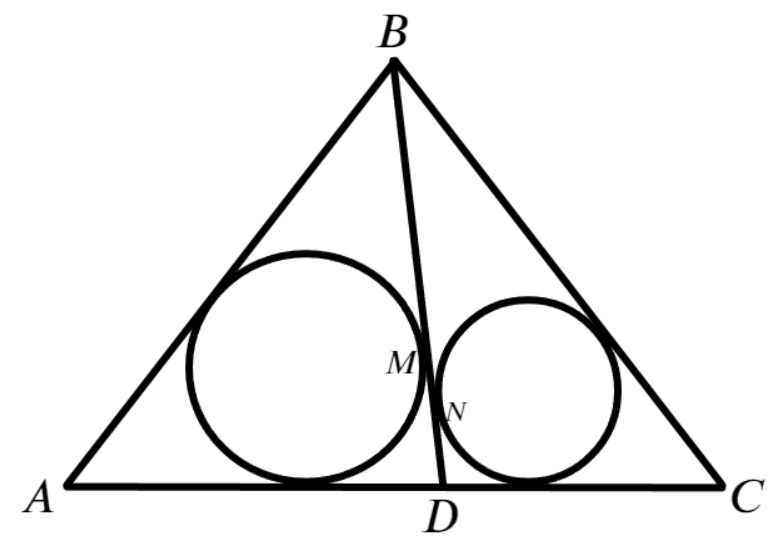
\includegraphics[scale=0.35]{g9-164.png}}
\end{figure}\\
По формуле для расстояния от вершины треугольника до точки касания имеем соотношения $DM=\cfrac{AD+BD-AB}{2},\ DN=\cfrac{CD+BD-BC}{2},$ тогда\\
$MN=DM-DN=\cfrac{AD+BD-AB}{2}-\cfrac{CD+BD-BC}{2}=\cfrac{AD-CD}{2}=\cfrac{4-3}{2}=\cfrac{1}{2}.$\\
